\documentclass[tikz,border=12pt]{standalone}
\usepackage[T1]{fontenc}
\usepackage{mathpazo}
\usepackage{amsmath,amssymb}
\usetikzlibrary{arrows.meta, calc}

\definecolor{stblue}{HTML}{7B97AD}
\definecolor{rwgold}{HTML}{B8995E}
\definecolor{sage}{HTML}{7A9A7E}
\definecolor{dkbrown}{HTML}{3D3530}
\definecolor{wmgray}{HTML}{7B7067}
\definecolor{cream}{HTML}{F9F6F0}
\definecolor{border}{HTML}{D4C9B8}
\definecolor{terracotta}{HTML}{C47A6A}
\definecolor{lavender}{HTML}{907EA0}

\begin{document}
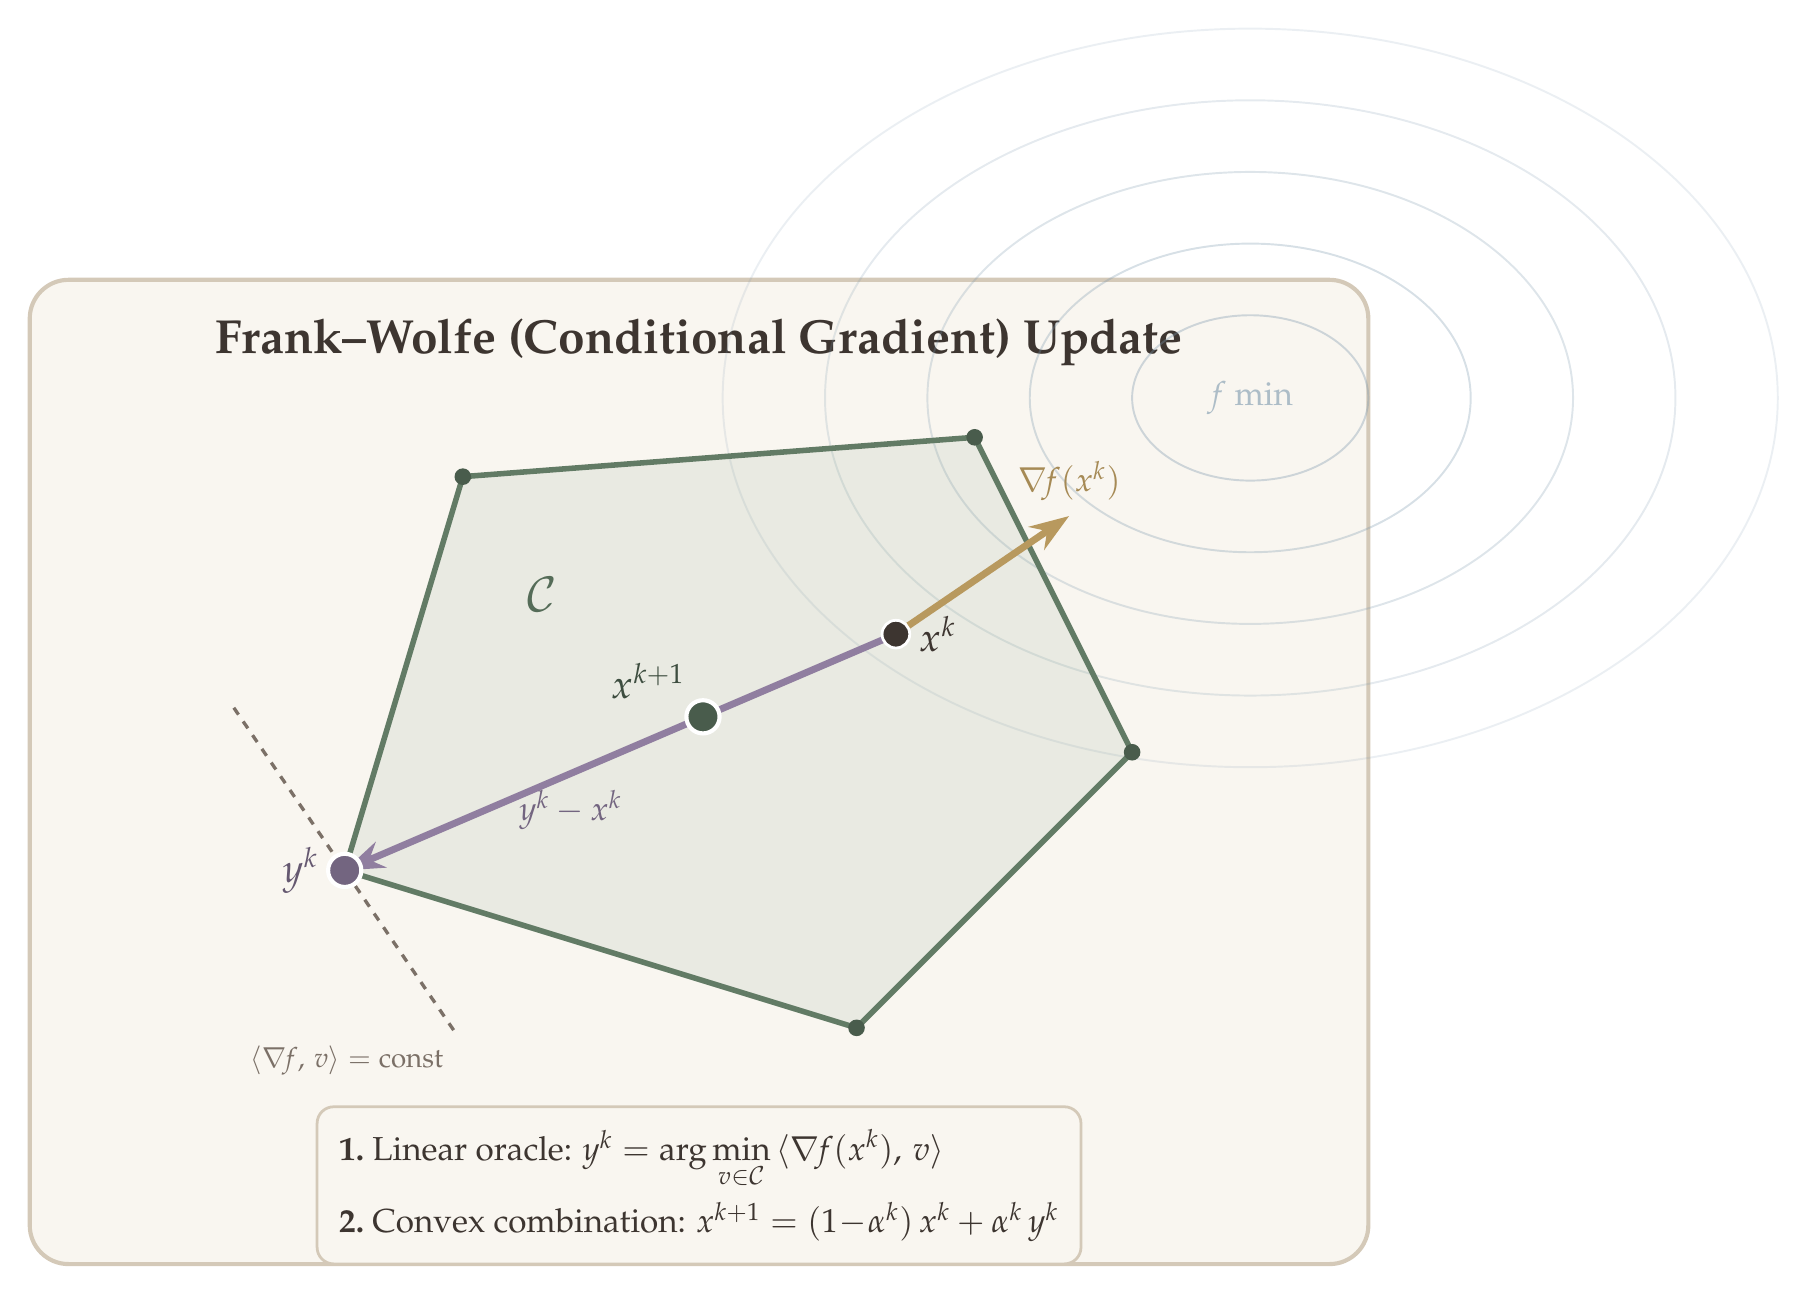
\begin{tikzpicture}[>={Stealth[length=4mm, width=3mm]}]

% Background
\fill[cream, rounded corners=14pt] (-3.5,-3.0) rectangle (13.5,9.5);
\draw[border, line width=1.5pt, rounded corners=14pt] (-3.5,-3.0) rectangle (13.5,9.5);

% Title
\node[text=dkbrown, font=\LARGE\bfseries] at (5.0,8.7)
  {Frank--Wolfe (Conditional Gradient) Update};

% Contour lines of f (centered upper-right, outside C)
\foreach \r/\op in {1.5/0.35, 2.8/0.30, 4.1/0.25, 5.4/0.20, 6.7/0.15} {
  \draw[stblue, line width=0.7pt, opacity=\op]
    (12.0,8.0) ellipse ({\r*1.0} and {\r*0.7});
}
\node[text=stblue, font=\large, opacity=0.6] at (12.0,8.0) {$f$ min};

% Convex polytope C (pentagon — asymmetric for generality)
\coordinate (v1) at (2.0,7.0);   % upper-left
\coordinate (v2) at (8.5,7.5);   % upper-right
\coordinate (v3) at (10.5,3.5);  % right
\coordinate (v4) at (7.0,0.0);   % lower-right
\coordinate (v5) at (0.5,2.0);   % lower-left

\fill[sage, opacity=0.12] (v1) -- (v2) -- (v3) -- (v4) -- (v5) -- cycle;
\draw[sage!80!black, line width=2pt] (v1) -- (v2) -- (v3) -- (v4) -- (v5) -- cycle;

% Vertex dots (small, to show polytope structure)
\foreach \v in {v1,v2,v3,v4,v5} {
  \fill[sage!60!black] (\v) circle (3pt);
}

% Label C
\node[text=sage!70!black, font=\LARGE\bfseries] at (3.0,5.5) {$\mathcal{C}$};

% === Key geometry ===
% x^k: inside C, upper-right region
\coordinate (xk) at (7.5,5.0);

% Gradient direction: pointing toward upper-right (toward unconstrained min)
\coordinate (gradtip) at ($(xk)+(2.2,1.5)$);

% y^k: the vertex that minimizes <grad f, v> — most anti-aligned with gradient
% Gradient points upper-right, so y^k is the lower-left vertex
\coordinate (yk) at (v5);  % (0.5, 2.0)

% x^{k+1}: convex combination, about 35% from x^k toward y^k
\coordinate (xk1) at ($(xk)!0.35!(yk)$);

% --- Step 1: Show gradient at x^k ---
\draw[rwgold, line width=2.5pt, -{Stealth[length=5mm, width=3.5mm]}]
  (xk) -- (gradtip);
\node[text=rwgold!90!black, font=\large\bfseries, above=2pt]
  at (gradtip) {$\nabla\!f(x^k)$};

% --- Supporting hyperplane at y^k (perpendicular to gradient) ---
% Normal to gradient direction is (-1.5, 2.2), normalized and scaled
\pgfmathsetmacro{\hlen}{2.5}
\pgfmathsetmacro{\nx}{-1.5}
\pgfmathsetmacro{\ny}{2.2}
\pgfmathsetmacro{\nrm}{sqrt(\nx*\nx+\ny*\ny)}
\coordinate (h1) at ($(yk)+(\nx/\nrm*\hlen, \ny/\nrm*\hlen)$);
\coordinate (h2) at ($(yk)-(\nx/\nrm*\hlen, \ny/\nrm*\hlen)$);
\draw[wmgray, line width=1.2pt, dashed] (h1) -- (h2);
\node[text=wmgray, font=\normalsize, below left=1pt] at (h2)
  {$\langle \nabla\!f,\, v \rangle = \mathrm{const}$};

% --- Step 2: FW direction arrow (from x^k toward y^k, full length) ---
\draw[lavender, line width=2.5pt, -{Stealth[length=5mm, width=3.5mm]}]
  (xk) -- (yk);
\node[text=lavender!80!black, font=\large\bfseries, below=6pt, xshift=-8pt]
  at ($(xk)!0.55!(yk)$) {$y^k - x^k$};

% --- Step 3: Convex combination (x^{k+1} on the segment) ---
% Highlight the segment from x^k to y^k with a thin line (already drawn by the arrow)
% Mark x^{k+1} prominently

% --- Points (on top) ---
% y^k (vertex, drawn first so FW arrow is under it)
\fill[lavender!80!black] (yk) circle (6pt);
\draw[white, line width=1.5pt] (yk) circle (6pt);
\node[text=lavender!70!black, font=\Large\bfseries, left=6pt] at (yk)
  {$y^k$};

% x^k
\fill[dkbrown] (xk) circle (5pt);
\draw[white, line width=1pt] (xk) circle (5pt);
\node[text=dkbrown, font=\Large\bfseries, right=5pt] at (xk) {$x^k$};

% x^{k+1}
\fill[sage!60!black] (xk1) circle (6pt);
\draw[white, line width=1.5pt] (xk1) circle (6pt);
\node[text=sage!50!black, font=\Large\bfseries, above left=3pt] at (xk1) {$x^{k+1}$};

% --- Annotation box ---
\node[text=dkbrown, font=\large,
      fill=cream, inner sep=8pt, align=left,
      draw=border, line width=1pt, rounded corners=6pt]
  at (5.0,-2.0)
  {\textbf{1.}\ Linear oracle: $y^k = \displaystyle\arg\min_{v \in \mathcal{C}}\,
   \langle \nabla\!f(x^k),\, v \rangle$\\[4pt]
   \textbf{2.}\ Convex combination: $x^{k+1} = (1\!-\!\alpha^k)\,x^k + \alpha^k\,y^k$};

\end{tikzpicture}
\end{document}
